\documentclass[12pt, a4paper, twoside]{scrreprt}

\usepackage[T1]{fontenc}
\usepackage{fixltx2e}
\usepackage{cmbright}
%\usepackage{lmodern}
\usepackage{amsmath,amsfonts,amssymb}
\usepackage{longtable,booktabs}
\usepackage{dcolumn}
\newcolumntype{.}{D{.}{.}{-1}}

\usepackage[numbers,sort&compress,elide]{natbib}

\usepackage{listings}

\usepackage{tikz}
\usetikzlibrary{shapes,arrows}

\tikzstyle{block} = [rectangle, minimum width=5.5em, minimum height=2em, draw = black, fill = blue!60!green!40, text width=4em, text centered, rounded corners]
\tikzstyle{drift} = [rectangle, minimum width=5.5em, minimum height=2em, draw = black, fill = red!100!blue!50!green!20, text width=4em, text centered, rounded corners]
\tikzstyle{line} = [draw, -latex']

\usepackage[parfill]{parskip}

\usepackage{fancyhdr}
\pagestyle{fancy}
\fancyhf{}
\addtolength{\headheight}{2.5pt}
\fancyhead[LO,RE]{\thepage}
\fancyhead[RO,LE]{\nouppercase{\leftmark}}
\renewcommand{\headrulewidth}{0.5pt}
\renewcommand{\footrulewidth}{0pt}
\renewcommand{\textfraction}{0.05}

\usepackage{graphicx}

\usepackage{appendix}

\setcapindent{0.05\textwidth}
\usepackage[labelfont=bf,labelsep=space]{caption}
\usepackage{subfig}
\usepackage{float}

\usepackage{geometry}
\geometry{a4paper,left=25mm,right=25mm, top=20mm, bottom=25mm}
\linespread{1.06}\selectfont
\widowpenalty=300
\clubpenalty=300

\usepackage{lscape}

\usepackage{color}

\definecolor{Black}{RGB}{0,0,0}

\definecolor{Grey}{RGB}{190,190,190}
\definecolor{DarkGrey}{RGB}{160,160,160}

\definecolor{DarkBlue}{RGB}{0,0,139}
\definecolor{RoyalBlue}{RGB}{65,105,225}
\definecolor{MediumBlue}{RGB}{0,0,205}
\definecolor{SkyBlue}{RGB}{135,206,235}
\definecolor{LightBlue}{RGB}{173,216,230}

\definecolor{DarkRed}{RGB}{139,0,0}
\definecolor{Gold}{RGB}{255,215,0}
\definecolor{Orange}{RGB}{255,165,0}
\definecolor{DarkOrange}{RGB}{192,64,0}

\definecolor{DarkGreen}{RGB}{0,100,0}
\definecolor{ForestGreen}{RGB}{34,139,34}
\definecolor{Olive}{RGB}{160,128,32}
\definecolor{DarkOliveGreen}{RGB}{85,107,47}

\definecolor{Purple}{RGB}{160,32,240}
\definecolor{Plum}{RGB}{221,160,221}
\definecolor{DarkPlum}{RGB}{144,80,64}

\lstset{
  basicstyle=\small\ttfamily,
  columns=flexible,
  frame=lines,
  framesep=10pt,
  keywordstyle=\color{DarkBlue},
  commentstyle=\ttfamily \color{DarkGreen},
  stringstyle=\color{DarkRed} 
}


\usepackage[colorlinks, linkcolor=black, anchorcolor=black, citecolor=black, urlcolor=black ]{hyperref}


\title{Garfield\kern-0.02em+\kern-0.02em+ User Guide}

\begin{document}
%\maketitle
\begin{titlepage}
  {
  \centering
  \sffamily
  \linespread{1.5}

  \vspace{3cm} 

  \huge{\textbf{Garfield++ User Guide}}

  \vspace{2cm}

  
\includegraphics[width=0.2\textwidth]{garfield.jpg}

  \vspace{2cm}

  \large
  Version 2017.2 

  \vspace{2cm}
  \large
  H. Schindler

  \vfill

  February 2017

  }
\end{titlepage}

\cleardoublepage
\tableofcontents
\cleardoublepage

\chapter{Introduction}

Garfield++ is an object-oriented toolkit for the detailed simulation of 
particle detectors which use a gas 
or a semiconductor material as sensitive medium. 

Garfield++ currently offers 3 techniques for calculating electric fields:
\begin{itemize}
  \item
  solutions in the thin-wire limit for devices made of wires and planes;
  \item
  an interface with the Ansys finite element program, 
  which can compute approximate fields in nearly arbitrary 
  two- and three-dimensional configurations 
  with dielectrics and conductors;
  \item
  an interface with the Synopsys Sentaurus device simulation program.
\end{itemize}

In the future, the program should become interfaced with neBEM, 
as is already the case for Garfield \cite{GarfieldFortran}.

\chapter{Getting Started}\label{Chap:Installation}

\section{Installation}

The source code is hosted on a Subversion\footnote{
For more information about Subversion, 
have a look at \url{http://svn.web.cern.ch/svn/docs.php} and the 
documents listed there.} (svn) repository 
managed by the CERN Central SVN service.
A web interface for browsing the code is available at: \\
\url{http://svnweb.cern.ch/world/wsvn}.

\begin{itemize}
  \item
  Define an environment variable \texttt{GARFIELD\_HOME} 
  pointing to the directory where the Garfield++ classes 
  are to be located.
  In the following, we assume that we want to install Garfield 
  in a directory \texttt{/home/mydir/garfield}.
  If you are using bash, type
  \begin{lstlisting}
export GARFIELD_HOME=/home/mydir/garfield
  \end{lstlisting}
  (replace \texttt{/home/mydir/garfield} by the path of your choice).
  For (t)csh-type shells, type
  \begin{lstlisting}
setenv GARFIELD_HOME /home/mydir/garfield
  \end{lstlisting}
  Include the above lines also in the \texttt{.bashrc} 
  (or \texttt{.cshrc}) file in your home directory. 
  If unsure which shell you are using, 
  type \texttt{echo \${SHELL}}.
  \item
  Download (``check out'') the code from the repository.
  This can be done via SSH access or via HTTP access.
  For SSH access, give the command
  \begin{lstlisting}
svn co svn+ssh://<username@>svn.cern.ch/reps/garfield/trunk $GARFIELD_HOME
  \end{lstlisting}
  For HTTPS access, give the command
  \begin{lstlisting}
svn co https://<username@>svn.cern.ch/reps/garfield/trunk $GARFIELD_HOME
  \end{lstlisting}
  Alternatively, if you do not want to use svn or do not have 
  a CERN afs account, 
  you can download the tarballs from the web interface 
  (see the above address) and extract them in the 
  \texttt{\$GARFIELD\_HOME} directory.
  \item
  Change to the \texttt{\${GARFIELD\_HOME}} directory 
  (\texttt{cd \$GARFIELD\_HOME}).
  \item 
  If necessary, adapt the \texttt{makefile} according 
  to your configuration. 
  By default, \texttt{gfortran} is used as Fortran compiler. 
  In order to use a different compiler (e. g. \texttt{g77}), 
  you can modify the definition of the variable \texttt{\$FC} in the 
  \texttt{makefile} accordingly.
  \item
  Compile the classes by giving the command \texttt{make}.
  \item
  Heed requires an environment variable \texttt{HEED\_DATABASE}
  to be defined.
  \begin{lstlisting}
export HEED_DATABASE=$GARFIELD_HOME/Heed/heed++/database/
  \end{lstlisting}
  Add this line also to your \texttt{.bashrc}/\texttt{.cshrc} as well.
\end{itemize}

After the initial ``check-out'', the command 
\begin{lstlisting}
svn update
\end{lstlisting}
followed by \texttt{make} 
(in case of trouble: try \texttt{make clean; make}),
can be used for downloading the latest version of the code 
from the repository.

%\subsection{GarfRoot}
%
%The Garfield++ classes can be used interactively within the ROOT shell.
%
\lstset{language=C++}

\section{Structure}

Garfield++ provides essentially a collection of classes 
which can be used as building blocks of 
a user program. 

An overview of the different types of classes is given in 
Fig.~\ref{Fig:OverviewClasses}. 
Two main categories can be distinguished: 
classes for describing the detector 
(material properties, geometry, fields), 
and transport classes which deal with the tracking of particles 
through the device. 
The two class types are linked by the class \texttt{Sensor}.

\begin{figure}
  \centering  
  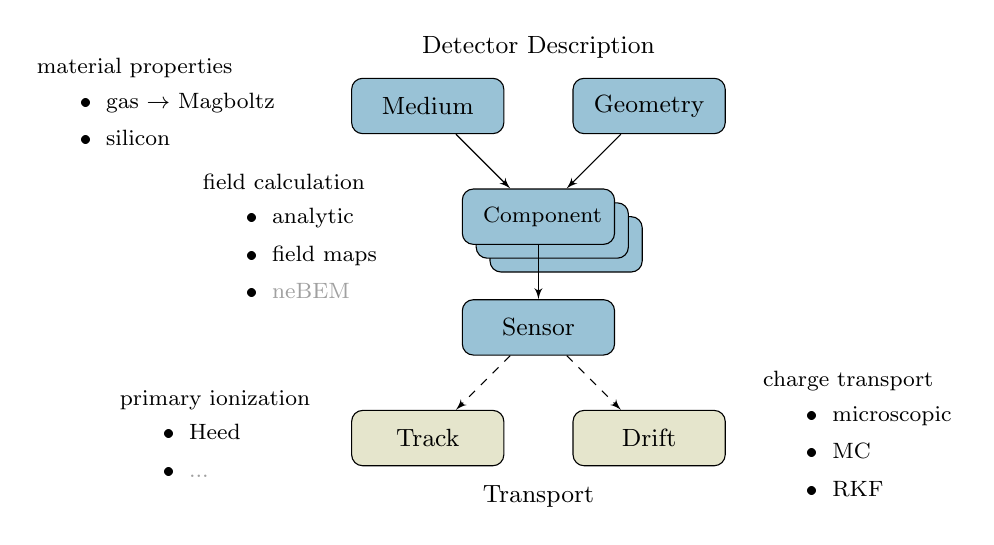
\begin{tikzpicture}[scale=2, node distance = 4em, 
                      auto, label distance = 1em]

    \node (medium) [block,
                    label=left:{\parbox{10em}{
                    \footnotesize material properties 
                    \begin{itemize} 
                      \item gas \(\rightarrow\) Magboltz 
                      \item silicon 
                    \end{itemize}}}]  {\small Medium};
    \node (dummy)  [right of=medium,
                    label=above:{\small Detector Description}] {};
    \node (geo)    [block,right of = dummy]  {\small Geometry};
    \node (comp1)  [block, below of = dummy, 
                    xshift = 1em, yshift = -1em]     {};
    \node (comp2)  [block, below of = dummy,
                    xshift =.5em,yshift=-.5em]   {};
    \node (comp)   [block, below of = dummy,
                    label=left:{\parbox{8em}{
                    \footnotesize \vspace{2em} 
                    field calculation 
                    \begin{itemize} 
                      \item analytic 
                      \item field maps 
                      \item \textcolor{DarkGrey}{neBEM} 
                    \end{itemize}}}]  {\footnotesize Component};
    \node (sensor) [block, below of = comp]  {\small Sensor};
    \node (dummy1) [below of = sensor,
                    label=below:{\small Transport}] {};
    \node (aval)   [drift, right of=dummy1,label=right:{\parbox{7em}{\footnotesize charge transport \begin{itemize} \item microscopic \item MC \item RKF \end{itemize}}}]        {\small Drift};
    \node (track)  [drift, left of=dummy1,label=left:{\parbox{7em}{\footnotesize primary ionization \begin{itemize} \item Heed \item \textcolor{DarkGrey}{...} \end{itemize}}}]      {\small Track}; 
    \path [line]   (medium) -- (comp);
    \path [line]   (geo)    -- (comp);
    \path [line]   (comp)   -- (sensor);
    \path [line,dashed]  (sensor) -- (track);
    \path [line,dashed]  (sensor) -- (aval);
  \end{tikzpicture}
  \caption{Overview of the main classes in Garfield\kern-0.05em+\kern-0.05em+ and their interplay.}
  \label{Fig:OverviewClasses}
\end{figure}

The individual classes are explained in detail in the following chapters. 

Readers familiar with the structure 
of (Fortran) Garfield \cite{GarfieldFortran} will recognize a 
rough correspondence between 
the above classes and the sections of Garfield. 
\texttt{Medium} classes, for instance, can be regarded as the counterpart 
of the \texttt{\&GAS} section; 
\texttt{Component} classes are similar in 
scope to the \texttt{\&CELL} section.  
 
Garfield\kern-0.05em+\kern-0.05em+ also includes a number of classes for visualization purposes, 
e. g. for plotting drift lines, making a contour plot of the electrostatic 
potential or inspecting the layout of the detector.   
These classes rely extensively on the graphics classes of the 
ROOT framework \cite{ROOT}.

\section{Examples}

\subsection{Drift Tube}

\subsubsection{Gas Table}
As a first step, we have to prepare a table of transport parameters 
(drift velocity, diffusion coefficients, Townsend coefficient,
and attachment coefficient) as a function 
of the electric field \(\mathbf{E}\)  
(and, in general, also the magnetic field \(\mathbf{B}\) 
as well as the angle between \(\mathbf{E}\) and \(\mathbf{B}\)).
In this example, we use a gas mixture of 93\% argon and 7\% 
carbon dioxide at a pressure of 3~atm and room temperature.
\begin{lstlisting}
MediumMagboltz* gas = new MediumMagboltz();
gas->SetComposition("ar", 93., "co2", 7.);
// Set temperature [K] and pressure [Torr].
gas->SetPressure(3 * 760.);
gas->SetTemperature(293.15);
\end{lstlisting} 
We also have to specify the number of electric fields to be 
included in the table and the electric field range to be covered. 
Here we use 20 field points between 100~V/cm and 100~kV/cm 
with logarithmic spacing. 
\begin{lstlisting}
gas->SetFieldGrid(100., 100.e3, 20, true);
\end{lstlisting}
Now we run Magboltz to generate the gas table for this grid. 
As input parameters we have to specify the number of collisions 
(in multiples of \(10^{7}\)) over which the electron is traced 
by Magboltz.
To see the full Magboltz output, we switch on debugging.
\begin{lstlisting}
gas->EnableDebugging();
gas->GenerateGasTable(10);
gas->DisableDebugging();
\end{lstlisting}
This calculation will take a while, so don't panic. 
After the calculation is finished, we save the gas table to a 
file for later use.
\begin{lstlisting}
gas->WriteGasFile("ar93_co2_7.gas");
\end{lstlisting}

\subsubsection{Electric Field}
For calculating the electric field inside the tube, 
we use the class \texttt{ComponentAnalyticField} which can handle 
(two-dimensional) arrangements of wires, planes and tubes. 
First we build the geometry, that is a list of volumes and associated 
media.
\begin{lstlisting}
// Wire radius [cm]
const double rWire = 25.e-4;
// Outer radius of the tube [cm]
const double rTube = 1.46;
// Half-length of the tube [cm]
const double lTube = 10.;
GeometrySimple* geo = new GeometrySimple();
// Make a tube (centered at the origin, inner radius: rWire, outer radius: rTube).
SolidTube* tube = new SolidTube(0., 0., 0., rWire, rTube, lTube);
// Add the solid to the geometry, together with the medium inside.
geo->AddSolid(box, gas); 
\end{lstlisting}

Next we setup the electric field.
\begin{lstlisting}
ComponentAnalyticField* cmp = new ComponentAnalyticField();
cmp->SetGeometry(geo);
// Voltages
const double vWire = 3270.;
const double vTube =    0.;
// Add the wire in the center.
cmp->AddWire(0., 0., 2 * rWire, vWire, 's');
// Add the tube.
cmp->AddTube(rTube, vTube, 0, 't');
\end{lstlisting}

Finally we assemble a \texttt{Sensor} object which acts as an 
interface to the transport classes discussed below.
\begin{lstlisting}
Sensor* sensor = new Sensor();
sensor->AddComponent(cmp);
\end{lstlisting}

\subsection{GEM}

\chapter{Media}\label{Chap:Media}

Media are derived from the abstract base class \texttt{Medium}.

The name (identifier) of a medium can be read by the function
\begin{lstlisting}
std::string GetName();
\end{lstlisting}
For compound media (e. g. gas mixtures), 
the identifiers and fractions of the constituents are available via
\begin{lstlisting}
int GetNumberOfComponents();
void GetComponent(const int, std::string label, double& f);
\end{lstlisting} 

\section{Transport Parameters}

\texttt{Medium} classes provide functions for calculating the 
macroscopic transport 
parameters of electrons, holes, and ions as a function of the 
electric and magnetic field:
\begin{lstlisting}
bool ElectronVelocity(const double ex, const double ey, const double ez,
                      const double bx, const double by, const double bz,
                      double& vx, double& vy, double& vz);
bool ElectronDiffusion(const double ex, const double ey, const double ez,
                       const double bx, const double by, const double bz,
                       double& dl, double& dt);
bool ElectronTownsend(const double ex, const double ey, const double ez,
                      const double bx, const double by, const double bz,
                      double& alpha);
bool ElectronAttachment(const double ex, const double ey, const double ez,
                        const double bx, const double by, const double bz,
                        double& eta);
\end{lstlisting}
\begin{description}
  \item[ex, ey, ez] electric field (in V/cm)
  \item[bx, by, bz] magnetic field (in T)
  \item[vx, vy, vz] drift velocity (in cm/ns)
  \item[dl, dt] longitudinal and transverse diffusion coefficients 
     (in \(\sqrt{\text{cm}}\))
  \item[alpha] Townsend coefficient (in \(\text{cm}^{-1}\))
  \item[eta] attachment coefficient (in \(\text{cm}^{-1}\))
\end{description}

The above functions return \texttt{true} if the respective parameter 
is available at the requested field.  

Analogous functions are available for holes 
(although of course not meaningful for gases), and also for ions 
(except for the Townsend and attachment coefficients). 
A function specific to ions is
\begin{lstlisting}
bool IonDissociation(const double ex, const double ey, const double ez,
                     const double bx, const double by, const double bz,
                     double& diss);
\end{lstlisting}
It returns the dissociation coefficient (in cm\(^{-1}\)). 

The components of the drift velocity are stored in a coordinate system 
which is aligned with the electric and magnetic field vectors.
More precisely, the axes are along
\begin{itemize}
  \item
  the electric field \(\mathbf{E}\),
  \item
  the component of the magnetic field \(\mathbf{B}\) transverse to 
  \(\mathbf{E}\), 
  \item
  \(\mathbf{E} \times \mathbf{B}\).
\end{itemize}
The longitudinal diffusion is measured along \(\mathbf{E}\).
The transverse diffusion is the average of the diffusion coefficients 
along the two remaining axes.

\begin{table}
  \centering
  \begin{tabular}{l r}
    \toprule
    transport parameter & scaling \\
    \midrule
    drift velocity & \(v\) vs. \(E/p\) \\
    diffusion      & \(\sigma\sqrt{p}\) vs. \(E/p\) \\
    Townsend coefficient & \(\alpha / p\) vs. \(E/p\) \\
    attachment coefficient & \(\eta / p\) vs. \(E/p\) \\ 
    \bottomrule
  \end{tabular}
  \caption{Pressure scaling relations for gases.}
  \label{Tab:PressureScaling}
\end{table}

\subsection{Transport Tables}

The transport parameters can either be stored in a 
one-dimensional table (as a function of the electric field only) or 
in a three-dimensional table (as a function of \textbf{E}, \textbf{B}, 
and the angle \(\theta\) between \textbf{E} and \textbf{B}). 
If only a one-dimensional table is present and the 
drift velocity at \(B \ne 0\) is requested, the Laue-Langevin equation 
is used. 

In the present version of the code,
all transport parameters share the same grid 
of electric fields, magnetic fields, and angles.
By default, the field and angular ranges are
\begin{itemize}
  \item
  20 electric field points between 100 V/cm and 100 kV/cm, 
  with logarithmic spacing
  \item
  \(\mathbf{B} = 0\), \(\phi = \pi / 2\)
\end{itemize}

For specifying the field grid, two functions are available:
\begin{lstlisting}
void SetFieldGrid(double emin, double emax, int ne, bool logE,
                  double bmin, double bmax, int nb,
                  double amin, double amax, int na);
void SetFieldGrid(const std::vector<double>& efields,
                  const std::vector<double>& bfields,
                  const std::vector<double>& angles);
\end{lstlisting}
\begin{description}
\item[emin, emax] min. and max. value of the electric field range to be covered by the tables
\item[ne] number of electric field grid points
\item[logE] flag specifying whether the \(E\)-field grid points should be 
evenly spaced (\texttt{false}), or logarithmically spaced (\texttt{true}) 
\item[bmin, bmax, ne] magnetic field range and number of values
\item[amin, amax, na] angular range and number of angles
\item[efields, bfields, angles] lists of \(E\), \(B\), and 
\(\theta\) (in ascending order)
\end{description}
Electric fields have to be supplied in V/cm, magnetic fields in Tesla, 
and angles in rad.

The gas tables are interpolated using Newton polynomials. 
The order of the interpolation polynomials can be set by means of
\begin{lstlisting}
void SetInterpolationMethodVelocity(const int intrp);
void SetInterpolationMethodDiffusion(const int intrp);
void SetInterpolationMethodTownsend(const int intrp);
void SetInterpolationMethodAttachment(const int intrp);
void SetInterpolationMethodIonMobility(const int intrp);
void SetInterpolationMethodIonDissociation(const int intrp);
\end{lstlisting}
\begin{description}
\item[intrp]
order of the interpolation polynomial 
\end{description}
The interpolation order must be between 1 and the smallest of the two 
numbers: 10 and number of table entries - 1. 
Orders larger than 2 are not recommended.

The method for extrapolating to \(E\) values smaller and larger 
than those present in the table can be set using 
\begin{lstlisting}
void SetExtrapolationMethodVelocity(const std::string extrLow,
                                    const std::string extrHigh);
\end{lstlisting}
\begin{description}
\item[extrLow, extrHigh] extrapolation method to be used 
(``constant'', ``exponential'', or ``linear'')
\end{description}
Similar functions are available for the other transport parameters. 
The extrapolation method set using this function has no effect on 
extrapolation in 3-dimensional tables. 
In such tables, polynomial extrapolation is performed with the same 
order as for the interpolation.

The default settings are
\begin{itemize}
  \item
  quadratic interpolation,
  \item
  constant extrapolation towards low values,
  \item
  linear extrapolation towards high values.
\end{itemize}

\section{Gases}

There are currently two classes implemented which can be used for the 
description of gaseous media: \texttt{MediumGas} and its 
daughter class \texttt{MediumMagboltz}. 
While \texttt{MediumGas} deals only with the interpolation of gas tables 
and the import of gas files, 
\texttt{MediumMagboltz} - owing to an interface to the 
Magboltz program \cite{Biagi1999} - allows the calculation 
of transport parameters. 
In addition, the latter class provides access to the 
electron-molecule scattering cross-sections used in Magboltz and is 
thus suitable for microscopic tracking (chapter \ref{Chap:Transport}). 

The composition of the gas mixture is specified using
\begin{lstlisting}
bool SetComposition(const std::string gas1, const double f1 = 1.,
                    const std::string gas2 = "", const double f2 = 0.,
                    const std::string gas3 = "", const double f3 = 0.,
                    const std::string gas4 = "", const double f4 = 0.,
                    const std::string gas5 = "", const double f5 = 0.,
                    const std::string gas6 = "", const double f6 = 0.);
\end{lstlisting}
\begin{description}
  \item[gas1, \dots, gas6] identifier of the molecule/atom
  \item[f1, \dots, f6] fraction of the respective molecule/atom   
\end{description}
A valid gas mixture comprises at least one and at most six 
different species. 
A list of the presently available gases and their identifiers 
can be found in the appendix. 
The fractions have to be strictly positive and 
may add up to any non-zero value; 
internally they will be normalized to 1.

The gas density is specified in terms of pressure (Torr) 
and temperature (K):
\begin{lstlisting}
void SetPressure(const double p);
void SetTemperature(const double t);
\end{lstlisting}
Note that the density is calculated using the ideal gas law. 

In the following example the gas mixture is set 
to Ar/CH\(_{4}\) (80/20) at 
atmospheric pressure and 20\(^{\circ}\)~C.
\begin{lstlisting}
MediumMagboltz* gas = new MediumMagboltz();
// Set the composition
gas->SetComposition("ar", 80., "ch4", 20.);
gas->SetTemperature(293.15);
gas->SetPressure(760.);
\end{lstlisting}

\subsection{Magboltz}

Magboltz, written by Steve Biagi, is a program \cite{Biagi1999} 
for the calculation of electron transport properties in gas 
mixtures using semi-classical Monte Carlo simulation. 
It includes a database of electron-atom/molecule cross-sections 
for a large number of detection gases. 

\texttt{MediumMagboltz} allows running Magboltz for a 
given electric field, magnetic field and field angle:
\begin{lstlisting}
void RunMagboltz(const double e, const double b, const double btheta,
                 const int ncoll, bool verbose, 
                 double& vx, double& vy, double& vz,
                 double& dl, double& dt, double& alpha, double& eta,
                 double& vxerr, double& vyerr, double& vzerr,
                 double& dlerr, double& dterr,
                 double& alphaerr, double& etaerr, 
                 double& alphatof);
\end{lstlisting}
\begin{description}
  \item[e, b, btheta] 
    \(\mathbf{E}\) field, \(\mathbf{B}\) field, and  angle
  \item[ncoll] 
    number of collisions (in multiples of \(10^{7}\)) over which 
    the electron is tracked
  \item[verbose] 
    flag switching on/off full output from Magboltz
  \item[vx, vy, vz] 
    drift velocity along \(\mathbf{E}\) (\(vz\)), 
    along \(\mathbf{B}_{t}\) (\(vy\)), and  
    along \(\mathbf{E} \times \mathbf{B}\) (\(vy\))
  \item[dl, dt]
    diffusion coefficients
  \item[alpha, eta]
    Townsend and attachment coefficient calculated using the
    SST technique or, at low fields, the ionization/loss rate
  \item[vxerr, vyerr, \dots, etaerr] 
    statistical error of the calculation in \(\%\)
  \item[alphatof]
    alternative estimate of the effective Townsend coefficient 
    \(\alpha - \eta\) based on Time-Of-Flight method  
\end{description}
The max. energy of the cross-section table  
is chosen automatically by Magboltz. 
For inelastic gases, setting \(\texttt{nColl} = 2 \dots 5\)
should give an accuracy of about \(1\%\). 
An accuracy better than \(0.5\%\) can be achieved by 
\(\texttt{nColl} > 10\). 
For pure elastic gases such as Ar, \texttt{nColl} should 
be at least 10.  
 
In order to calculate the electron transport parameters 
for all values of \(\mathbf{E}\), \(\mathbf{B}\), 
and \(\theta\) included in the current field grid, 
the function
\begin{lstlisting}
void GenerateGasTable(const int numCollisions);
\end{lstlisting}
can be used.
 
Electron transport parameter tables can be saved to file 
and read from file  
by means of
\begin{lstlisting}
bool WriteGasFile(const std::string filename);
bool LoadGasFile(const std::string filename);
\end{lstlisting}

The format of the gas file used in Garfield++ is compatible with the 
one used in Garfield 9. 

\subsection{Functions for Microscopic Tracking}


\section{Semiconductors}

\chapter{Components}\label{Chap:Components}

The calculation of electric fields is done by \texttt{Component} classes. 
The key functions of \texttt{Component} classes are 
\begin{lstlisting}
  void ElectricField(const double x, const double y, const double z,
                     double& ex, double& ey, double& ez,
                     Medium*& m, int& status);
  void ElectricField(const double x, const double y, const double z,
                     double& ex, double& ey, double& ez, double& v);
  Medium* GetMedium(const double& x, const double& y, const double& z);
\end{lstlisting}
\begin{description}
  \item[x, y, z] 
  position where the electric field (medium) is to be determined
  \item[ex, ey, ez, v] 
  electric field and potential at the given position
  \item[m] pointer to the medium at the given position; 
  if there is no medium at this location, a null pointer is returned
  \item[status] status flag indicating where the point is located
  (see Table~\ref{Tab:StatusFlagsField})
\end{description}
The function \texttt{GetMedium} returns \texttt{true} if a medium was found at the given location. 

\begin{table} 
  \centering
  \begin{tabular}{l l}
  \toprule
  value & meaning \\
  \midrule
    0   & inside a drift medium \\
  \(> 0\) & inside a wire \\
   -1 \dots -4  &  on the side of a plane where no wires are \\
   -5   & inside the mesh, but not in a drift medium \\
   -6   & outside the mesh \\
  \bottomrule
  \end{tabular}
  \caption{Status flags for electric fields.}
  \label{Tab:StatusFlagsField}
\end{table}

\section{Defining the Geometry}

As mentioned above, the purpose of \texttt{Component} classes is to 
provide, for a given location, the electric (and magnetic) field and a pointer to the 
\texttt{Medium} (if available).
For the latter task, it is obviously necessary to specify the geometry 
of the device. 
In case of field maps, the geometry is already fixed in the field solver. 
It is, therefore, sufficient to associate the materials 
defined in the field map with the corresponding \texttt{Medium} classes. 

For other components (e. g. analytic or user-parameterized fields), 
the geometry has to be defined separately. 

Simple structures can be described by the native geometry (\texttt{GeometrySimple}), which has only a very restricted repertoire of shapes (solids). 
At present, the available solids are
\begin{itemize}
  \item
  \texttt{SolidBox}
  \item
  \texttt{SolidTube}
\end{itemize} 

As an example, we consider a gas-filled tube with a diameter of 1~cm and 
a length of 20~cm (along the \(z\)-axis), centered at the origin:
\begin{lstlisting}
// Create the medium.
MediumMagboltz* gas = new MediumMagboltz();
// Create the geometry.
GeometrySimple* geo = new GeometrySimple();
// Dimensions of the tube
double rMin = 0., rMax = 0.5, halfLength = 10.;
SolidTube* tube = new SolidTube(0., 0., 0., rMin, rMax, halfLength);
// Add the solid to the geometry, together with the gas inside.
geo->AddSolid(tube, gas);
\end{lstlisting}
Solids may overlap. 
When the geometry is scanned 
(triggered, for instance, by calling \texttt{GetMedium}), the  
first medium found is returned. 
The sequence of the scan is reversed with respect to the 
assembly fo the geometry. 
Hence, the last medium added to the geometry is considered the innermost. 

For more complex structures, the class \texttt{GeometryRoot} can be used 
which provides an interface to the ROOT geometry (\texttt{TGeo}).
Using \texttt{GeometryRoot}, the above example would look like this:
\begin{lstlisting}
// Create the ROOT geometry.
TGeoManager* geoman = new TGeoManager("world", "geometry");
// Create the ROOT material and medium. 
// For simplicity we use the predefined material "Vacuum".
TGeoMaterial* matVacuum = new TGeoMaterial("Vacuum", 0, 0, 0);
TGeoMedium*   medVacuum = new TGeoMedium("Vacuum", 1, matVacuum);
// Dimensions of the tube
double rMin = 0., rMax = 0.5, halfLength = 10.;
// In this simple case, the tube is also the top volume.
TGeoVolume* top = geoman->MakeTube("TOP", medVacuum, rMin, rMax, halfLength);
geoman->SetTopVolume(top);
geoman->CloseGeometry();
// Create the Garfield medium.
MediumMagboltz* gas = new MediumMagboltz();
// Create the Garfield geometry.
GeometryRoot* geo = new GeometryRoot();
// Pass the pointer to the TGeoManager.
geo->SetGeometry(geoman);
// Associate the ROOT medium with the Garfield medium.
geo->SetMedium("Vacuum", gas); 
\end{lstlisting} 

In either case (\texttt{GeometrySimple} and \texttt{GeometryRoot}),
after assembly the geometry is passed to the \texttt{Component} as a pointer:
\begin{lstlisting}
void SetGeometry(GeometryBase* geo);
\end{lstlisting}

\subsection{Visualization}

Geometries described by \texttt{GeometrySimple} can be viewed 
using the class \texttt{ViewGeometry}. 
For example, let us assume that \texttt{geo} is a class instance of 
\texttt{GeometrySimple}. 
\begin{lstlisting}
// Create a viewer.
ViewGeometry* view = new ViewGeometry();
// Set the pointer to the geometry.
view->SetGeometry(geo);
view->Plot();
\end{lstlisting}

ROOT geometries can be viewed by calling the \texttt{Draw()} function of
\texttt{TGeoManager}. 

The layout of an arrangement of wires, planes and tubes
defined in \texttt{ComponentAnalyticField} 
can be inspected using the class \texttt{ViewCell}.

Let \texttt{component} be a class instance of \texttt{ComponentAnalyticField}.
\begin{lstlisting}
// Create a viewer.
ViewCell* view = new ViewCell();
// Set the pointer to the component.
view->SetComponent(component);
// Make a two-dimensional plot of the cell layout.
view->Plot2d();
\end{lstlisting}
Similarly, the function \texttt{ViewCell::Plot3d()} creates 
a three-dimensional view of the cell layout.

\section{Field Maps}

\subsection{Ansys}

The interpolation of FEM field maps 
created with the program Ansys \cite{ANSYS} 
is dealt with by the classes
\texttt{ComponentAnsys121} and \texttt{ComponentAnsys123}. 
The class names refer to the type of mesh element used by Ansys:
  \begin{itemize}
  \item
  \texttt{ComponentAnys121} reads two-dimensional field maps 
with 8-node curved quadrilaterals (known as ``plane121'' in Anys). 
  \item
  \texttt{ComponentAnsys123} reads three-dimensional field maps 
with quadric curved tetrahedra (known as ``solid123'' in Ansys).
  \end{itemize}
The field map is imported with the function
\begin{lstlisting}
  bool Initialise(std::string elist, std::string nlist,
                  std::string mplist, std::string prnsol,
                  std::string unit);
\end{lstlisting}
\begin{description}
  \item[elist]
  name of the file containing the list of elements 
  (default: \texttt{"ELIST.lis"})
  \item[nlist]
  name of the file containing the list of nodes
  (default: \texttt{"NLIST.lis"})
  \item[mplist]
  name of the file containing the list of materials
  (default: \texttt{"MPLIST.lis"})
  \item[prnsol]
  name of the file containing the nodal solutions
  (default: \texttt{"PRNSOL.lis"})
  \item[unit]
  length unit used in the calculation (default: \texttt{"cm"}, \\ 
  other recognized units are 
  \texttt{"mum"}/\texttt{"micron"}/\texttt{"micrometer"},
  \texttt{"mm"}/\texttt{"millimeter"} and 
  \texttt{"m"}/\texttt{"meter"}).
\end{description}
The return value is \texttt{true} if the map was successfully read. 

In order to enable charge transport and ionization,
the materials in the map need to be associated with \texttt{Medium} classes.
\begin{lstlisting}
// Get the number of materials in the map
int GetNumberOfMaterials();
// Associate a material with a Medium class
void SetMedium(const int imat, Medium* medium);
\end{lstlisting}
\begin{description}
\item[imat]
index in the list of (field map) materials
\item[medium]
pointer to the \texttt{Medium} class to be associated with this material
\end{description}

The materials in the field map are characterized by the 
relative dielectric constant \(\varepsilon\) and the 
conductivity \(\sigma\). 
These parameters are accessible through the functions
\begin{lstlisting}
double GetPermittivity(const int imat);
double GetConductivity(const int imat);
\end{lstlisting}

A weighting field map can be imported using
\begin{lstlisting}
bool SetWeightingField(std::string prnsol, std::string label);
\end{lstlisting}
\begin{description}
  \item[prnsol]
  name of the file containing the nodal solution for the weighting field
  configuration
  \item[label]
  arbitrary name, used for identification of the electrode/signal
\end{description}

The weighting field map has to use the same mesh as the previously 
read ``actual'' field map.

For periodic structures, e. g. GEMs, one usually models only 
the basic cell of the geometry and applies appropriate symmetry 
conditions to cover the whole problem domain. 
The available symmetry operations are:
\begin{itemize}
  \item
  simple periodicities,
  \item
  mirror periodicities, 
  \item
  axial periodicities, and
  \item
  rotation symmetries.
\end{itemize}

Mirror periodicity and simple periodicity as well as 
axial periodicity and rotation symmetry are, 
obviously, mutually exclusive. 
In case of axial periodicity, the field map has to cover an 
integral fraction of \(2\pi\). 

Periodicities can be set and unset using
\begin{lstlisting}
void EnablePeriodicityX();       void DisablePeriodicityX();
void EnableMirrorPeriodicityX(); void DisableMirrorPeriodicityX();
void EnableAxialPeriodicityX();  void DisableAxialPeriodicityX();
void EnableRotationSymmetryX();  void DisableRotationSymmetryX();
\end{lstlisting}
Analogous functions are available for \(y\) and \(z\).

In order to assess the quality of the mesh, 
one can retrieve the dimensions of each mesh element using
\begin{lstlisting}
GetElement(const int i, double& vol, double& dmin, double& dmax);
\end{lstlisting}
\begin{description}
\item[i] index of the element
\item[vol] volume/area of the element
\item[dmin, dmax] min./max. distance between two node points
\end{description}

In the following example we make histograms of the aspect ratio and 
element size.
\begin{lstlisting}
ComponentAnsys123* fm = new ComponentAnsys123();
...
TH1F* hAspectRatio = new TH1F("hAspectRatio"; "Aspect Ratio", 100, 0., 50.);
TH1F* hSize = new TH1F("hSize", "Element Size", 100, 0., 30.);
const int nel = fm->GetNumberOfElements();
// Loop over the elements.
double volume, dmin, dmax;
for (int i = nel; i--;) {
  fm->GetElement(i, volume, dmin, dmax);
  if (dmin > 0.) hAspectRatio->Fill(dmax / dmin);
  hSize->Fill(volume);
}
TCanvas* c1 = new TCanvas();
hAspectRatio->Draw();
TCanvas* c2 = new TCanvas();
c2->SetLogy();
hSize->Draw();
\end{lstlisting}

\subsection{Synopsys TCAD}

Electric fields calculated using the device simulation program 
Synopsys Sentaurus \cite{Synopsys} can be imported with the classes 
\texttt{ComponentTcad2d} and \texttt{ComponentTcad3d}.

The function to import the field map is 
\begin{lstlisting}
bool Initialise(const std::string gridfilename,
                const std::string datafilename);
\end{lstlisting}
\begin{description}
  \item[gridfilename]
  name of the mesh file, the extension is typically \texttt{.grd}
  \item[datafilename]
  name of the file containing the nodal solution;
  the filename typically typically ends with \texttt{\_des.dat}
\end{description}

Both files have to be exported in DF-ISE format, 
files in the default TDR format cannot be read.
The classes have been tested with meshes created with the application 
\texttt{Mesh} which can produce axis-aligned 
two- and three-dimensional meshes.
The only three-dimensional mesh elements \texttt{ComponentTcad3d} 
can deal with are tetrahedra. 
A mesh which consists only of simplex elements 
(triangles in 2D, tetrahedra in 3D), 
can be generated by invoking \texttt{Mesh} with the option \texttt{-t}.

After importing the files, 
the regions of the device where charge transport is to be enabled 
need to be associated with \texttt{Medium} classes. 
\begin{lstlisting}
// Get the number of regions in the device
int GetNumberOfRegions();
// Associate a region with a Medium class
void SetMedium(const int ireg, Medium* m);
\end{lstlisting}
\begin{description}
  \item[ireg]
  index in the list of device regions
  \item[medium]
  pointer to the \texttt{Medium} class to be associated with this region
\end{description}

The name of a region can be retrieved with
\begin{lstlisting}
void GetRegion(const int i, std::string& name, bool& active);
\end{lstlisting}
\begin{description}
  \item[name] 
  label of the region as defined in the device simulation
  \item[active] 
  flag indicating whether charge transport is enabled 
  in this region
\end{description}

Simple periodicities and mirror periodicities along 
\(x\), \(y\), and - in case of \texttt{ComponentTcad3d} - \(z\) 
are supported. 
\begin{lstlisting}
void EnablePeriodicityX();
void EnableMirrorPeriodicityX();
\end{lstlisting}

\section{Analytic Fields}

For two-dimensional geometries consisting of wires, planes and tubes, 
analytic solutions are available.


\subsection{Description of the Cell}

Wires, tubes and planes can be added to the cell layout by means of the 
following functions:
\begin{lstlisting}
// Add a wire
void AddWire(const double x, const double y, const double d,
             const double v, const char label, 
             const double length = 100.,
             const double tension = 50., const double rho = 19.3);
// Add a tube
void AddTube(const double r, const double v, 
             const int nEdges, const char label);
// Add a plane at constant x
void AddPlaneX(const double x, const double v, const char label);
// Add a plane at constant y
void AddPlaneY(const double y, const double v, const char label);

\end{lstlisting} 

In all of these functions, the potential \texttt{v} (in V) 
and a label (used for signal calculation) 
have to be supplied as parameters.
 
For wires, the center of the wire (\texttt{x, y}) 
and its diameter (\texttt{d}) need to be specified. 
Optional parameters are the wire length, the tension (more precisely, the 
mass in g of the weight used to stretch the wire during the assembly) and 
the density (in g/cm\(^{3}\)) of the wire material. 
These parameters have no influence on the electric field. 
The number of wires which can be added is not limited.

Tube-specific parameters are the radius\footnote{For non-circular tubes, this parameter is the distance between the origin and any of the edges.} (\texttt{r}) and the number of edges, which determines the shape of the tube:
  \begin{itemize}
    \item
    \(n = 0\): cylindrical pipe
    \item
    \(3 \le n \le 8\): regular polygon 
  \end{itemize}
There can be only one tube in a cell. 
The tube is always centered at the origin \(\left(0, 0\right)\).

Planes are described by their coordinates. 
A cell can have at most two \(x\) and two \(y\) planes. 
Planes and tubes cannot be used together in the same cell.

The geometry can be reset (thereby deleting all wires, planes and tubes) by
\begin{lstlisting}
void Clear();
\end{lstlisting}

Before assembling and inverting the capacitance matrix, 
a check is performed whether the provided geometry matches the requirements.
If necessary, the planes and wires are reordered. 
Wires outside the tube or the planes as well as overlapping wires are removed.

\subsection{Periodicities}
The class supports simple periodicity in \(x\) and \(y\) direction.
The periodic lengths are set by means of
\begin{lstlisting}
void SetPeriodicityX(const double s);
void SetPeriodicityY(const double s);
\end{lstlisting}

\subsection{Cell Types}

Internally, cells are classified as belonging to one of these types:
\begin{description}
  \item[A]
  non-periodic cells with a most one \(x\) and one \(y\) plane
  \item[B1X]
  \(x\)-periodic cells without \(x\) planes and at most one \(y\) plane
  \item[B1Y]
  \(y\)-periodic cells without \(y\) planes and at most one \(x\) plane
  \item[B2X]
  cells with two \(x\) planes and at most one \(y\) plane
  \item[B2Y]
  cells with two \(y\) planes and at most one \(x\) plane
  \item[C1]
  doubly periodic cells without planes
  \item[C2X]
  doubly periodic cells with \(x\) planes
  \item[C2Y]
  doubly periodic cells with \(y\) planes
  \item[C3]
  doubly periodic cells with \(x\) and \(y\) planes
  \item[D1]
  round tubes without axial periodicity
  \item[D2]
  round tubes with axial periodicity
  \item[D3]
  polygonal tubes without axial periodicity
\end{description}

After the cell has been assembled and initialized, the cell type can be 
retrieved by the function
\begin{lstlisting}
std::string GetCellType();
\end{lstlisting}

\section{Other Components}

For simple calculations, \texttt{ComponentConstant} can be used. 
As the name implies, it provides a uniform electric field. 
The electric field and potential can be specified using
\begin{lstlisting}
void SetElectricField(const double ex, const double ey, const double ez);
void SetPotential(const double x, const double p, const double z,
                  const double v);
\end{lstlisting}
\begin{description}
  \item[ex, ey, ez]
  components of the electric field
  \item[x, y, z]
  coordinates where the potential is specified
  \item[v]
  voltage at the given position
\end{description}

The class \texttt{ComponentUser} takes the electric field and potential
from a user-defined function.
\begin{lstlisting}
void SetElectricField(void (*f)(const double, const double, const double, 
                                double& double&, double&));
void SetPotential(void (*f)(const double, const double, const double, 
                            double&));
\end{lstlisting}
\begin{description}
  \item[f] pointer to the user function
\end{description}

As an example, let us consider the field in an overdepleted diode, 
given by
\begin{equation*}
E\left(x\right) = \frac{V - V_{\text{dep}}}{d} + 
                    2x \frac{V_{\text{dep}}}{d^{2}},
\end{equation*}
where \(V\) is the applied bias voltage, \(V_{\text{dep}}\) is 
the depletion voltage, and \(d\) is the thickness of the diode.
\begin{lstlisting}
void efield(const double x, const double y, const double z,
            double& ex, double& ey, double& ez) {

  // Depletion voltage
  const double vdep = 160.;
  // Applied voltage
  const double v = 200.;
  // Detector thickness
  const double d = 0.1;

  ey = ez = 0.;
  ex = (v - vdep) / d + 2 * x * vdep / (d * d);

}

ComponentUser* component = new ComponentUser();
component->SetElectricField(efield);

\end{lstlisting}

\section{Visualizing the Field}

The class \texttt{ViewField} provides a number of functions 
for plotting the potential and field of a component. 
\begin{lstlisting}
void PlotContour();
void PlotSurface();
void PlotProfile(const double x0, const double y0, const double z0,
                 const double x1, const double y1, const double z1);
\end{lstlisting}
\begin{description}
  \item[x0, \dots, z1]
  coordinates of the start and end points of the line along which 
  the potential is to be evaluated
\end{description}

The first two functions create a contour and surface plot, respectively, 
of the potential in the selected viewing plane. 
The latter function plots the potential along the line  
\(\left(x_{0}, y_{0}, z_{0}\right) \rightarrow 
  \left(x_{1}, y_{1}, z_{1}\right)\).

The viewing plane and the region to be drawn 
can be specified using
\begin{lstlisting}
void SetArea(double xmin, double ymin,
             double xmax, double ymax);
void SetPlane(double fx, double fy, double fz,
              double x0, double y0, double z0);
void Rotate(double angle);
\end{lstlisting}

The density of the plotting grid can be set using
\begin{lstlisting}
void SetNumberOfSamples1d(const int n);
void SetNumberOfSamples2d(const int nx, const int ny);
\end{lstlisting}
\begin{description}
  \item[n, nx, ny]
  number of points in \(x\) and \(y\) direction 
  (default for one-dimensional plots: \(n = 1000\);
   default for two-dimensional plots: \(n_{x} = n_{y} = 200\)) 
\end{description}

The number of contour levels can be set using
\begin{lstlisting}
void SetNumberOfContours(const int n);
\end{lstlisting}

\section{Sensor}

The \texttt{Sensor} class can be viewed as a composite of components. 
In order to obtain a complete description of a detector, 
it is sometimes useful to combine fields from different 
\texttt{Component} classes.
For instance, one might wish to use a field map for the electric field, 
calculate the weighting field using analytic methods, 
and use a parameterized \(B\) field. 
Superpositions of several electric, magnetic and weighting fields are also possible. 


Components are added using
\begin{lstlisting}
void AddComponent(ComponentBase* comp);
void AddElectrode(ComponentBase* comp, std::string label);
\end{lstlisting}
While \texttt{AddComponent} tells the \texttt{Sensor} that the 
respective \texttt{Component} should be included in the calculation 
of the electric and magnetic field, 
\texttt{AddElectrode} requests the weighting field named \texttt{label} 
to be used for computing the corresponding signal.

To reset the sensor, thereby removing all components and electrodes, use
\begin{lstlisting}
void Clear();
\end{lstlisting}

The total electric and magnetic fields 
(sum over all components) at a given position are accesible through 
the functions \texttt{ElectricField} and \texttt{MagneticField}.
The syntax is the same as for the corresponding functions of the 
\texttt{Component} classes.
Unlike the fields, materials cannot overlap. 
The function \texttt{Sensor::GetMedium}, therefore, 
returns the first valid drift medium found. 
 
The \texttt{Sensor} acts as an interface to the transport classes.

For reasons of efficiency, it is sometimes useful to restrict 
charge transport, ionization and similar calculations to a 
certain region of the detector.
This ``user area'' can be set by
\begin{lstlisting}
void SetArea(double xmin, double ymin, double zmin,
             double xmax, double ymax, double zmax);
\end{lstlisting} 
\begin{description}
\item[xmin, \dots, zmax]
corners of the bounding box within which transport is enabled. 
Calling \texttt{SetArea()} (without arguments) sets the 
user area to the envelope of all components (if available).

\end{description}
In addition, the \texttt{Sensor} class takes care of 
signal calculations (discussed in chapter \ref{Chap:Signals}).
\chapter{Tracks}\label{Chap:Tracks}

The purpose of classes of the type \texttt{Track} is to simulate  
ionization patterns produced by fast charged particles traversing the detector. 

The type of the primary particle is set by the function
\begin{lstlisting}
void SetParticle(std::string particle);
\end{lstlisting}
\begin{description}
  \item[particle]
  name of the particle 
\end{description}
Only particles which are sufficiently long lived to leave a 
track in a detector are considered.
A list of the available particles is given 
in Table~\ref{Tab:ParticleNames}.

The kinematics of the charged particle can be defined 
by means of a number of equivalent methods:
  \begin{itemize}
    \item
    the total energy (in eV) of the particle,
    \item
    the kinetic energy (in eV) of the particle,
    \item
    the momentum (in eV/\(c\)) of the particle,
    \item
    the (dimension-less) velocity \(\beta = v / c\), 
    the Lorentz factor \(\gamma = 1 / \sqrt{1 - \beta^2}\) 
    or the product \(\beta\gamma\) of these two variables.
  \end{itemize}
The corresponding functions are
\begin{lstlisting}
void SetEnergy(const double e);
void SetKineticEnergy(const double ekin);
void SetMomentum(const double p);
void SetBeta(const double beta);
void SetGamma(const double gamma);
void SetBetaGamma(const double bg);
\end{lstlisting}

\begin{table}
  \centering
  \begin{tabular}{l l . r}
    \toprule
    particle & & \multicolumn{1}{c}{mass [MeV/\(c^{2}\)]} & charge \\
    \midrule
    \(e\)     & \texttt{electron, e-} & 0.510998910 & \(-1\) \\
    \(e^{+}\) & \texttt{positron, e+} & 0.510998910 & \(+1\) \\
    \(\mu^{-}\) & \texttt{muon, mu-}  & 105.658367  & \(-1\) \\
    \(\mu^{+}\) & \texttt{mu+}        & 105.658367  & \(+1\) \\
    \(\pi^{-}\) & \texttt{pion, pi, pi-} & 139.57018 & \(-1\) \\
    \(\pi^{+}\) & \texttt{pi+}           & 139.57018 & \(+1\) \\
    \(K^{-}\)   & \texttt{kaon, K, K-}   & 493.677   & \(-1\) \\
    \(K^{+}\)   & \texttt{K+}            & 493.677   & \(+1\) \\
    \(p\)       & \texttt{proton, p}     & 938.272013 & \(+1\) \\
    \(\overline{p}\) & \texttt{anti-proton, antiproton, p-bar} & 938.272013 & \(-1\) \\
    \(d\)       & \texttt{deuteron, d} & 1875.612793 & \(+1\) \\
  \bottomrule
  \end{tabular}
  \caption{Available charged particles.}
  \label{Tab:ParticleNames}
\end{table}

A track is initialized by means of
\begin{lstlisting}
void NewTrack(const double x0, const double y0, const double z0,
               const double t0,
               const double dx0, const double dy0, const double dz0);
\end{lstlisting}
\begin{description}
  \item[x0, y0, z0] initial position (in cm)
  \item[t0] starting time
  \item[dx0, dy0, dz0] initial direction vector
\end{description}
The starting point of the track has to be inside an ionizable medium. 
Depending on the type of \texttt{Track} class, there can be 
further restrictions on the type of \texttt{Medium}.
If the specified direction vector has zero norm, an isotropic random vector 
will be generated.
 
After successful initialization, the ``clusters'' produced along the track
can be retrieved by
\begin{lstlisting}
bool GetCluster(double& xcls, double& ycls, double& zcls, double& tlcs,
                int& n, double& e, double& extra);
\end{lstlisting}
\begin{description}
  \item[xcls, ycls, zcls, tcls] 
  position (and time) of the ionizing collision
  \item[n] number of electrons produced in the collision
  \item[e] transferred energy (in eV)
\end{description}
The function returns \texttt{false} if the list of clusters is exhausted
 or if there is no valid track.

The concept of a ``cluster'' deserves some explanation. 
In the present context it refers to the energy loss in a single ionizing 
collision of the primary charged particle and the secondary 
electrons produced in this process. 


\section{Heed}

The program Heed \cite{Smirnov2005} is an implementation 
of the photo-absorption ionization (PAI) model. 
It is written and maintained by I. Smirnov.
An interface to Heed is available through the class \texttt{TrackHeed}. 

After calling \texttt{GetCluster}, 
one can retrieve details about the 
electrons in the present cluster using
\begin{lstlisting}
bool GetElectron(const int i, double& x, double& y, double& z,
                 double& t, double& e, 
                 double& dx, double& dy, double& dz);
\end{lstlisting}

\subsection{Delta Electron Transport}

Heed simulates the energy degradation of \(\delta\) electrons and 
the production of secondary (``conduction'') electrons 
using a phenomenological algorithm described in \cite{Smirnov2005}.

The asymptotic \(W\) value (eV) and the Fano factor of a 
\texttt{Medium} can be specified by the user by means of the functions
\begin{lstlisting}
void Medium::SetW(const double w);
void Medium::SetFanoFactor(const double f);
\end{lstlisting}
If these parameters are not set, Heed uses internal default values. 
The default value for the Fano factor is \(F = 0.19\).

The transport of \(\delta\) electrons can be activated or deactivated 
using
\begin{lstlisting}
void EnableDeltaElectronTransport();
void DisableDeltaElectronTransport();
\end{lstlisting} 

If \(\delta\) electron transport is disabled, 
the number of electrons returned by \texttt{GetCluster} is 
the number of ``primary'' ionisation electrons, 
i. e. the photo-electrons and Auger electrons. 
Their kinetic energies and locations are accessible 
through the function \texttt{GetElectron}.

If \(\delta\) electron transport is enabled (default setting), 
the function \texttt{GetElectron} returns the 
locations of the ``conduction'' electrons as calculated by the 
internal \(\delta\) transport algorithm of Heed. 
Since this method does not provide the energy and direction of the 
secondary electrons, the corresponding parameters in 
\texttt{GetElectron} are not meaningful in this case. 

\subsection{Photon Transport}

Heed can also be used for the simulation of x-ray photoabsorption. 
\begin{lstlisting}
void TransportPhoton(const double x0, const double y0, const double z0,
                     const double t0, const double e0,
                     const double dx0, const double dy0, const double dz0,
                     int& nel);
\end{lstlisting}
\begin{description}
\item[x0, y0, z0, t0] initial position and time of the photon
\item[e0] photon energy in eV
\item[dx0, dy0, dz0] direction of the photon
\item[nel] number of photoelectrons and Auger-electrons produced 
           in the photon conversion
\end{description}

\chapter{Charge Transport}\label{Chap:Transport}

\begin{equation}\label{Eqn:FirstOrderEquationOfMotion}
  \dot{\mathbf{r}} = 
  \mathbf{v}_{\text{d}}\bigl(\mathbf{E}\left(\mathbf{r}\right), 
                             \mathbf{B}\left(\mathbf{r}\right)\bigr).
\end{equation}

The following methods are available:
\begin{itemize}
  \item
  microscopic transport (\texttt{AvalancheMicroscopic}),
  \item
  Monte Carlo integration of the equation of motion,
  using macroscopic transport parameters (\texttt{AvalancheMC}), and
  \item
  Runge-Kutta integration of the equation of motion,
  using macroscopic transport parameters (to be implemented).
\end{itemize}

\section{Runge-Kutta-Fehlberg Integration}

\section{Monte Carlo Integration}

\section{Microscopic Tracking}

Microscopic tracking is (at present) only possible for electrons. 

A calculation is started by means of
\begin{lstlisting}
void AvalancheElectron(const double x0, const double y0, const double z0,
                       const double t0, const double e0,
                       const double dx0 = 0., const double dy0 = 0., const double dz0 = 0.);
\end{lstlisting}
\begin{description}
  \item[x0, y0, z0, t0] initial position and time
  \item[e0] initial energy (eV)
  \item[dx0, dy0, dz0] initial direction 
\end{description}
If the norm of the direction vector is zero, 
the initial direction is randomized.

After the calculation is finished, the number of electrons 
(\texttt{ne}) and ions (\texttt{ni})  
produced in the avalanche can be retrieved using
\begin{lstlisting}
void GetAvalancheSize(int& ne, int& ni);
\end{lstlisting}
Information about the ``history'' of each avalanche electron can be 
retrieved by
\begin{lstlisting}
int GetNumberOfElectronEndpoints();
void GetElectronEndpoint(const int i, 
               double& x0, double& y0, double& z0, double& t0, double& e0,
               double& x1, double& y1, double& z1, double& t1, double& e1,
                 int& status); 
\end{lstlisting}
\begin{description}
  \item[i] index of the electron
  \item[x0, y0, z0, t0, e0] initial position, time and energy of the electron
  \item[x1, y1, z1, t1, e1] final position, time and energy of the electron
  \item[status] status code indicating why the tracking of the electron was stopped.  
\end{description}
A list of status codes is given in Table~\ref{Tab:DriftLineStatusCodes}.

\begin{table}
  \centering
  \begin{tabular}{r l}
    \toprule
    status code &  meaning\\
    \midrule
     -1 & particle left the drift area        \\
     -5 & particle not inside a drift medium  \\
     -7 & attachment                          \\
    -16 & energy below transport cut          \\
    -17 & outside the time window             \\
    \bottomrule
  \end{tabular}
  \caption{Status code for the termination of drift lines.}
  \label{Tab:DriftLineStatusCodes}
\end{table}

The electron energy distribution can be extracted in the following way:
\begin{lstlisting}
AvalancheMicroscopic* aval = new AvalancheMicroscopic();
// Make a histogram (100 bins between 0 and 100 eV).
TH1F* hEnergy = new TH1F("hEnergy", "Electron energy", 100, 0., 100.);
// Pass the histogram to the avalanche class.
aval->EnableElectronEnergyHistogramming(hEnergy);
\end{lstlisting} 
After each collision, 
the histogram is filled with the current electron energy. 

\chapter{Signals}\label{Chap:Signals}

Signals are calculated using the Shockley-Ramo theorem. 
The current \(i\left(t\right)\) induced by a particle with charge 
\(q\) at a position \(\mathbf{r}\) moving at a velocity \(\mathbf{v}\)
is given by
\begin{equation*}
  i\left(t\right) = -q \mathbf{v} \cdot \mathbf{E}_{w}\left(\mathbf{r}\right),
\end{equation*}
where \(\mathbf{E}_{w}\) is the so-called weighting field for the 
electrode to be read out. 

The basic steps to enable the calculation 
of induced signals in Garfield++ are
\begin{enumerate}
  \item
  Prepare the weighting field for the electrode to be read out. 
  This step depends on the field calculation which is used. 
  \item
  Tell the \texttt{Sensor} that you want to use this 
  weighting field for the signal calculation. 
  \begin{lstlisting}
sensor->AddElectrode(ComponentBase* cmp, std::string label);
  \end{lstlisting}
  where \texttt{cmp} is a pointer to the \texttt{Component} 
  which calculates the weighting field, and \texttt{label} is 
  the name you have assigned to the weighting field in the previous step.
  \item
  Setup the binning for the signal calculation.
  \begin{lstlisting}
Sensor::SetTimeWindow(const double tmin, const double tstep, 
                      const int nbins);
  \end{lstlisting}
  The first parameter in this function is the lower time limit (in ns), 
  the second one is the bin width (in ns), and the last one 
  is the number of time bins. 
  \item
  Switch on signal calculation in the transport classes using 
  \begin{lstlisting}
AvalancheMicroscopic::EnableSignalCalculation();
AvalancheMC::EnableSignalCalculation();
  \end{lstlisting}
  After that the \texttt{Sensor} accumulates the signals of all 
  avalanches and drift lines you calculate.
\end{enumerate}

\begin{appendix}

\chapter{Units and Constants}

The basic units are cm for distances, g for (macroscopic) masses, 
and ns for times. 
Particle energies, momenta and masses are expressed 
in eV, eV/c and eV/c\(^{2}\), respectively.
For example, the electron mass is given in eV/c\(^{2}\), 
whereas the mass density of a material is given in g/cm\(^{3}\). 
The mass of an atom is specified in terms of the atomic mass number \(A\).
  
There are two important deviations from this system of units.
\begin{itemize}
  \item
  The unit for the magnetic field \(\mathbf{B}\) corresponding
  to the above system of units  (10\(^{-5}\) Tesla) is impractical. 
  Instead, magnetic fields are expressed in Tesla.
  \item
  Pressures are specified in Torr.
  \item
  Electric charge is expressed in fC. 
\end{itemize}
A summary of commonly used quantities and their units is given 
in Table~\ref{Tab:Units}.
\begin{table}
  \centering
  \begin{tabular}{l l}
    \toprule
    physical quantity & unit \\
    \midrule
    length & cm \\
    mass & g \\
    time & ns \\
    temperature & K \\
    electric potential & V \\
    electric charge & fC \\
    \midrule
    energy & eV \\
    pressure & Torr \\
    electric field & V / cm \\
    magnetic field & Tesla \\
    electric current & fC / ns \\
    angle & rad \\
    \bottomrule
  \end{tabular}
  \caption{Physical units.}
  \label{Tab:Units}
\end{table}
  
The values of the physical constants used in the code are defined  
in the file \texttt{FundamentalConstants.hh}.

\chapter{Gases}

Table \ref{Tab:GasesMagboltz8} shows a list of the gases 
available in the current version of Magboltz. 
The star rating represents an estimate of the reliability 
of the cross-section data for the respective gas. 
A rating of ``5*'' indicates a detailed, well-validated 
description of the cross-sections, while 
``2*'' indicates a low quality, that is 
a coarse modelling of the cross-sections 
associated with large uncertainties.

\begin{longtable}{l l l}
  \toprule
   chem. symbol & name & rating \\
  \midrule
  \(^{4}\)He & helium   & 5* \\
  \(^{3}\)He & helium-3 & 5* \\
          Ne & neon     & 5* \\
          Ar & argon    & 5* \\
          Kr & krypton  & 4* \\
          Xe & xenon    & 4* \\
  \midrule
  Cs         & cesium   & 2* \\
  Hg         & mercury  & 2* \\
  \midrule
  H\(_{2}\) & hydrogen  & 5* \\
  D\(_{2}\) & deuterium & 5* \\
  N\(_{2}\) & nitrogen  & 5* \\
  O\(_{2}\) & oxygen    & 4* \\
  F\(_{2}\) & fluorine  & 2* \\
  \midrule
  CO         & carbon monoxide & 5* \\
  NO         & nitric oxide    & 4* \\
  \midrule
  H\(_{2}\)O & water           & 4* \\ 
  CO\(_{2}\) & carbon dioxide  & 5* \\
  N\(_{2}\)O & nitrous oxide   & 2* \\
  O\(_{3}\)  & ozone           & 3* \\
  H\(_{2}\)S & hydrogen sulfide & 2* \\
  COS        & carbonyl sulfide & 2* \\
  CS\(_{2}\) & carbon disulfide & 2* \\
  \midrule
  CH\(_{4}\)           & methane   & 5* \\
  CD\(_{4}\)           & deuterated methane & 4* \\
  C\(_{2}\)H\(_{6}\)   & ethane    & 5* \\
  C\(_{3}\)H\(_{8}\)   & propane   & 4* \\
  nC\(_{4}\)H\(_{10}\) & n-butane  & 4* \\
  iC\(_{4}\)H\(_{10}\) & isobutane & 4* \\ 
  nC\(_{5}\)H\(_{12}\) & n-pentane & 4* \\  
  neo-C\(_{5}\)H\(_{12}\) & neopentane & 4* \\
  C\(_{2}\)H\(_{4}\)   & ethene    & 4* \\
  C\(_{2}\)H\(_{2}\)   & acetylene & 4* \\
  C\(_{3}\)H\(_{6}\)   & propene   & 4* \\
  C\(_{3}\)H\(_{6}\)   & cyclopropane & 4* \\
  \midrule
  CH\(_{3}\)OH         & methanol        & 3* \\
  C\(_{2}\)H\(_{5}\)OH & ethanol         & 3* \\
  C\(_{3}\)H\(_{7}\)OH & isopropanol     & 3* \\
  C\(_{3}\)H\(_{8}\)O\(_{2}\)  & methylal & 2* \\
  C\(_{4}\)H\(_{10}\)O\(_{2}\) & DME      & 4* \\
  \midrule
  CF\(_{4}\)           & tetrafluoromethane & 5* \\
  CHF\(_{3}\)          & fluoroform         & 3* \\
  C\(_{2}\)F\(_{6}\)   & hexafluoroethane   & 4* \\
  C\(_{2}\)H\(_{2}\)F\(_{4}\) & tetrafluoroethane & 2* \\
  C\(_{3}\)F\(_{8}\)   & octafluoropropane  & 3* \\
  SF\(_{6}\)           & sulfur hexafluoride  & 3* \\
  BF\(_{3}\)           & boron trifluoride    & 4* \\ 
  CF\(_{3}\)Br         & bromotrifluoromethane & 3* \\
  \midrule
  NH\(_{3}\)           & ammonia  & 4* \\
  SiH\(_{4}\)          & silane   & 4* \\
  GeH\(_{4}\)          & germane  & 3* \\
  \bottomrule
  \caption{Gases available in Magboltz 8}
  \label{Tab:GasesMagboltz8}
\end{longtable}

\end{appendix}

\bibliographystyle{amsplain}
\bibliography{UserGuide}

\end{document}
